

\def\nameoflab{Temperature Trends in Sweden}
\def\coursecode{MNXB11}

\def\authorOne{Jens Hieronymus, Lukas Nord, Linn Preuss Jelvez}
\def\authorOneMail{}
\def\headerName{}

\def\supervisor{}
\def\supervisorMail{}

\documentclass[12pt,titlepage]{article}

\usepackage[utf8]{inputenc}


% Set your default font encoding.
\usepackage[T1]{fontenc}

% Set default language priority order.
\usepackage[english]{babel}

% Set default margins.
\usepackage[a4paper,margin=25mm,headsep=5mm,headheight=12pt]{geometry}

\usepackage{amsmath,amssymb,amsfonts,amsthm}  % Mathematics
%\usepackage{bbold}

\usepackage{hyperref} 
\hypersetup{colorlinks, 
    citecolor=black,
    filecolor=black, 
    linkcolor=black,
    urlcolor=black
      }

\usepackage{setspace}
\usepackage{graphicx}
\usepackage{subcaption}
%\usepackage[separate-uncertainty=true]{siunitx} %Use this for writing SI units
% \sisetup{
%   range-phrase=--,
%   detect-all,
%   output-decimal-marker={.},
%   range-units=single,
%   per-mode=reciprocal,
%   separate-uncertainty=false
% }
%\usepackage{physics} %A lot of useful short commands for writing math/physics
\usepackage{url}
\usepackage{verbatim}
%\usepackage[toc,acronym]{glossaries}
\usepackage{booktabs} % For nice tables
\usepackage{fancyhdr} % For header and footer
%\usepackage{lipsum}
%\usepackage{lastpage} % For page counter
%\usepackage{svg} % Makes it possible to use .svg files 
\usepackage{float} % Just [H] for placing figures
%\usepackage{comment} % Use \begin{comment}
\usepackage{listings} % Enables source code listings
\usepackage{enumerate}
\usepackage{enumitem}
% \definecolor{codegreen}{rgb}{0,0.75,0}
% \definecolor{codegray}{rgb}{0.5,0.5,0.5}
% \definecolor{codepurple}{rgb}{0.58,0,0.82}
% \definecolor{backcolour}{rgb}{0.97,0.96,0.97}
\lstdefinestyle{mystyle}{
    backgroundcolor=\color{backcolour},   
    commentstyle=\color{codegreen},
    keywordstyle=\color{codepurple},
    numberstyle=\tiny\color{codegray},
    stringstyle=\color{magenta},
    basicstyle=\ttfamily\footnotesize,
    breakatwhitespace=false,         
    breaklines=true,                 
    captionpos=b,                    
    keepspaces=true,                 
    numbers=left,                    
    numbersep=5pt,                  
    showspaces=false,                
    showstringspaces=false,
    showtabs=false,                  
    tabsize=2
}

\lstset{style=mystyle}

% using inkscapefiles
\graphicspath{{figures/}}

%\begin{comment}
%\usepackage{fontspec}

%\setmainfont{LTRemark}[
%    Path=./font/,
%    Extension = .otf,
%    UprightFont=*-Roman,
%    BoldFont=*-Bold,
%    ItalicFont=*-Italic,
%    BoldItalicFont=*-BoldItalic
%]
%\end{comment}

%\usepackage{tcolorbox}
% \definecolor{lightblue}{rgb}{0.85, 0.85, 0.98}
% \definecolor{darkblue}{rgb}{0.3, 0.3, 0.95}
% \newtcolorbox{mybox}[1]{
%     colback=lightblue,
%     colframe=darkblue,
%     fonttitle=\bfseries,
%     title=#1} 

% Use option lineno for line numbers 

\usepackage{float}
\usepackage{subcaption}
\usepackage{caption}
\usepackage{graphicx}




%\title{Temperature Trends in Sweden}

%\author[1]{Jens Hieronymus}
%\author[1]{Lukas Nord}
%\author[1]{Linn Preuss Jelvez}
%\affil[1]{Group 8}

\begin{document}
\begin{titlepage}
    \vspace*{\fill}	\newcommand{\HRule}{\rule{\linewidth}{0.5mm}}
	\center 
	\HRule\\[0.4cm]
	{\huge\bfseries \nameoflab}\\[0.4cm]
        {\Large\bfseries \coursecode}\\[0.1cm]
	\HRule\\[1.5cm]

    \large
    \textit{Author}\\
    \authorOne  \\ 

    \vspace{1cm}
     
    Lund University\\
    Department of Physics
     
    
    \bigbreak
    \vfill
    \today
\end{titlepage}

%\maketitle
% \begin{abstract}
% Please provide an abstract of no more than 300 words. Your abstract should explain the main contributions of your article, and should not contain any material that is not included in the main text. 
% \end{abstract}



\flushbottom

\thispagestyle{empty}

\section*{ABSTRACT}
Please provide an abstract of no more than 300 words. Your abstract should explain the main contributions of your article, and should not contain any material that is not included in the main text.

%\keywords{Solar Cycle, Climate, Birthdays}



\section{Introduction}

Everyone knows the weather, but few people have actually analyzed the data we publicly have access to. We decided to look at this data and see what could actually be inferred from it. We set out to do 3 investigations:
\begin{enumerate}
    \item Climate Trends
    \item Birthday Temperature Trends
    \item Solar Activity Period Estimation
\end{enumerate}

We are using the Swedish Meteorological and Hydrological Institute (SMHI), since that is the country we live in.

\subsection{Climate Trends}
We study how Sweden’s temperature has changed from 1850 to 2024 by analyzing trends in maximum, minimum, and mean temperatures for both the Lund station and the country as a whole to quantify the general climate trend.

\subsection{Birthday Temperature Trends}


{\Huge \textcolor{red}{We are born \\ and \\ We die}}\\\textcolor{red}{/Homer Simpson (perchance)}\\

We were curious to see how the temperature has historically changed over our birthdays [todo].

\subsection{Solar Activity Period Estimation}
The solar activity is usually measured by looking at the number of sunspots on the sun. Instead of this we wanted to see if this increase in activity, and thus luminosity would impact the temperature in Sweden and if this period could be inferred.

% Purpose: Briefly explain why studying temperature trends over long periods is important (e.g., climate change indicators, regional variation, etc.).

% Scope: Describe what the project investigates:

% Long-term mean temperature evolution in Sweden

% Temperature trends on specific calendar dates (e.g., birthdays)

% Possible correlations with solar events

% Data Source: SMHI open climate dataset (1850–2024).

\section{Data and Methods}

The data used in this project come from the Swedish Meteorological and Hydrological Institute (SMHI) and are provided as open datasets in CSV format, covering the years 1850–2024. Each file contains daily temperature measurements from several Swedish weather stations, along with metadata such as measurement quality indicators.

In the preprocessing stage, all data points flagged as low quality were removed using the provided quality information. Unnecessary metadata fields were also discarded to simplify the dataset. The cleaned data were then sorted into folders corresponding to the different parts of the analysis. The C++ analysis, discussed below, was performed on these filtered CSV files.

For efficient handling and statistical analysis, the processed CSV files were converted into \texttt{.root} files, which were then used for plotting and fitting in ROOT.

The entire workflow, from data filtering to final visualization, is automated using a set of Bash scripts.

\subsection{Climate Trends}
The climate trend analysis was performed by calculating the annual maximum, minimum, and mean temperatures for each weather station. The same calculations were then repeated using data from all stations combined to represent Sweden as a whole. The processed data was saved in CSV format and imported into ROOT, where the temperature trends were plotted and fitted with linear functions.

\subsection{Birthday Temperature Trends}
The analysis of the temperature on our birthdays began with filtering the data to keep only the correct days each year. To be able to compare the temperatures on our birthdays accurately, the data was filtered again to only include the temperature between times 10:00 and 15:00. This resulted in some days having more data points than others and an average was taken of all the temperatures for each day. Having the resulting data sorted in time, the next step was to group the points of each day to make it easier to plot them separately. The average temperature of each day was then plotted over time to compare the temperatures between the days and see how the average temperature on each day changes over time. 


\subsection{Solar Activity Period Estimation}
The analysis for the solar activity period estimation began by filtering the temperatures to be some time around midday (11:00 to 15:00 UTC), this was done in preparation for the next step. The next step was to adjust the temperatures based on what the expected solar output would be given the time, date and location. Filtering to times around midday allows for mitigation of some effects that would be caused by the atmosphere, as well as avoid times before sunrise and after sunset where the solar output would have been 0. With these adjusted temperatures, which essentially assume the sun is directly overhead, the next steps can be taken. This is described in the equations below.\\

The Equation of Time (EoT) quantifies the difference between solar time and mean clock time due to Earth's axial tilt and orbital eccentricity.  
It is given in minutes as:
\begin{align}
    B &= \frac{2\pi (J - 81)}{364} \label{eq:B} \\
    E_{\mathrm{oT}} &= 9.87 \sin(2B) - 7.53 \cos(B) - 1.5 \sin(B) \label{eq:EoT}
\end{align}
where \( J \) is the day of the year (\( J=1 \) for January 1). Where 81 is the approximate day of the year of the march equinox, and 364 is used instead of 365 to symmetrize the annual period.  \( B \) is the normalized angular position of earth in its orbit. The other numbers in the equation are derived from empirical data, on earths eccentricity as well as the behavior of the sun.\\

The solar declination angle \( \delta \) (in radians) is the angular position of the Sun north or south of the celestial equator:
\begin{equation}
    \delta = 23.45^\circ \times \frac{2\pi}{180^\circ} \times 
    \sin\!\left( B \right)
\end{equation}
where \(23.45^\circ\) is earths axial tilt.\\

Because Earth's orbit is slightly elliptical, the distance to the Sun varies through the year.  
The eccentricity correction factor \( E_0 \) adjusts the solar constant:
\begin{equation}
    E_0 = 1 + 0.033 \cos\!\left( \frac{2\pi J}{365} \right)
\end{equation}
where 0.033 is an estimate of earths eccentricity.\\

The local solar time (LST) in hours is given by
\begin{equation}
    \mathrm{LST} = h_{\mathrm{UTC}} + \frac{4\lambda + E_{\mathrm{oT}}}{60}
\end{equation}
where \(h_{\mathrm{UTC}}\) is the time given in the dataset, and \(\lambda\) is the longitude also from the dataset. The 4 comes from the fact that 4 minutes occur for every degree earth rotates(\(4 \frac{min}{^\circ}\), and the 60 converts that to hours.\\

The solar hour angle (in radians) is then
\begin{equation}
    H = 15^\circ  (\mathrm{LST} - 12)  \frac{2\pi}{180^\circ}
\end{equation}
where the \(15^\circ\) is the amount earth rotates per hour, and 12 is local noon on the local meridian.\\

The cosine of the solar zenith angle, \( \mu_0 = \cos\theta_z \), depends on the observer's latitude \( \varphi \), the solar declination \( \delta \), and the solar hour angle \( H \):
\begin{equation}
    \mu_0 = \sin\varphi \, \sin\delta + \cos\varphi \, \cos\delta \, \cos H
\end{equation}

The top-of-atmosphere (TOA) horizontal irradiance \( G_{0h} \) at UTC hour \(h_{\mathrm{UTC}}\) is
\begin{equation}
    G_{0h}(J, h_{\mathrm{UTC}}, \lambda, \varphi) =
    \begin{cases}
        I_{\mathrm{sc}} \, E_0 \, \mu_0, & \mu_0 > 0 \\
        0, & \text{otherwise.}
    \end{cases}
\end{equation}
where \(I_{\mathrm{sc}} \approx 1367\frac{W}{m^2}\) is the standard output of the sun at earths distance. This accounts for solar declination, local hour angle, and orbital effects.\\  
When \( \mu_0 \le 0 \), the Sun is below the horizon and no irradiance is received.\\

For a given year (with \( D = 365 \) or \( 366 \) days), the mean TOA irradiance for a fixed UTC hour is
\begin{equation}
    \bar{G}_{0h}(h_{\mathrm{UTC}}, \lambda, \varphi) =
    \frac{1}{D} \sum_{J=1}^{D} G_{0h}(J, h_{\mathrm{UTC}}, \lambda, \varphi)
\end{equation}

These 2 values are then subtracted and multiplied by a correlation factor \(\beta = 0.003 \frac{^\circ C m^2}{W}\) to arrive at the amount that would be subtracted from the temperature.
\begin{equation}
    t_{adj} = t_{data} - \beta(G_{0h}-\bar{G}_{0h})
\end{equation}
The value of \(\beta\) was chosen somewhat arbitrarily but another investigation would optimize it to minimize the variance of \(t_{adj}\) to eliminate atmospheric effects as much as possible. In such a case the next step can be skipped.\\

Next the data was compiled by day of year, so that for each day of the year, there were data-points for each location and year (time could be ignored at this point). This was used to normalize the data for each day to a value between 0 and 1. This was done so that temperatures between the days of year could be compared. Now these normalized values were averaged for each month over the data, this data was plotted. Then a fast fourier transform was done on this data to see which frequencies were dominant, this was also converted into periods to make it easier to examine.


\section{Research Question and Approach}

\subsection{Climate Trends}

We investigate how the temperature in Sweden has changed over time using historical data from 1850 to 2024. The analysis focuses on long-term trends in maximum, minimum, and mean temperatures, both for a single station in Lund and for Sweden as a whole. The goal is to determine whether there is a measurable long-term change and to quantify the trend that describes the evolution of the Swedish climate.

The temperature variation over time is approximated as a linear trend, and a linear fit is applied to estimate the rate of change. This fitted model also provides a simple way to project possible future temperature patterns.



\subsection{Birthday Temperature Trends}
We chose to investigate the temperature changes throughout time for specific days, spanning a period from 100 and 200 years ago up to the present. The goal was to find if the temperature of each day changed by a similar amount over the years and, if not, to identify when during the year the temperature changes the most. \\

To consider the different climates in the south and north of Sweden, we chose to study the temperatures in Lund and Luleå. 

\subsection{Solar Activity Period Estimation}
We use the temperature data across Sweden to see if the solar activity cycle period can be estimated. We adjust the temperature, normalize it and average it to get a timeseries of adjusted data.\\

We expect this time series to have a peak frequency in line with the known solar activity frequency.

\newpage
\section{Results, Discussion and Conclusion}

Here we present and discuss the findings for the different research questions mentioned above. Each research question is treated separately.

% 4.1 Long-Term Mean Temperature

% Plot(s) showing mean temperature over time.

% Linear fit with slope in °C per century.

% Comment on uncertainty or variability.

% 4.2 Birthday Trends

% Temperature trends for selected dates.

% Observations on seasonal or personal date differences.

% 4.3 Solar Event Analysis

% Visuals comparing temperature and solar activity.

% Note on whether patterns are correlated or independent.
\subsection{Long-Term Temperature Trends}

To investigate the long-term changes in climate, the maximum, minimum, and mean temperatures were analyzed over the period 1850--2024. Linear fits were applied to estimate the overall rate of temperature change in both individual stations and the combined Swedish dataset.


Figure \ref{fig:lund_maxmin} and \ref{fig:lund_mean} shows the temperature trends for the Lund station. The results show an increase in maximum temperature and a decrease in minimum temperature over the studied period. This implies that while summers have become warmer, winters or night-time temperatures have become colder. Consequently, the annual temperature range has widened, suggesting stronger variability. The mean annual temperature, however, still shows a slight positive linear trend, consistent with an overall gradual warming of approximately one degree per century.

\begin{figure}[H]
    \centering
%    \begin{subfigure}[b]{0.48\textwidth}
        \centering
        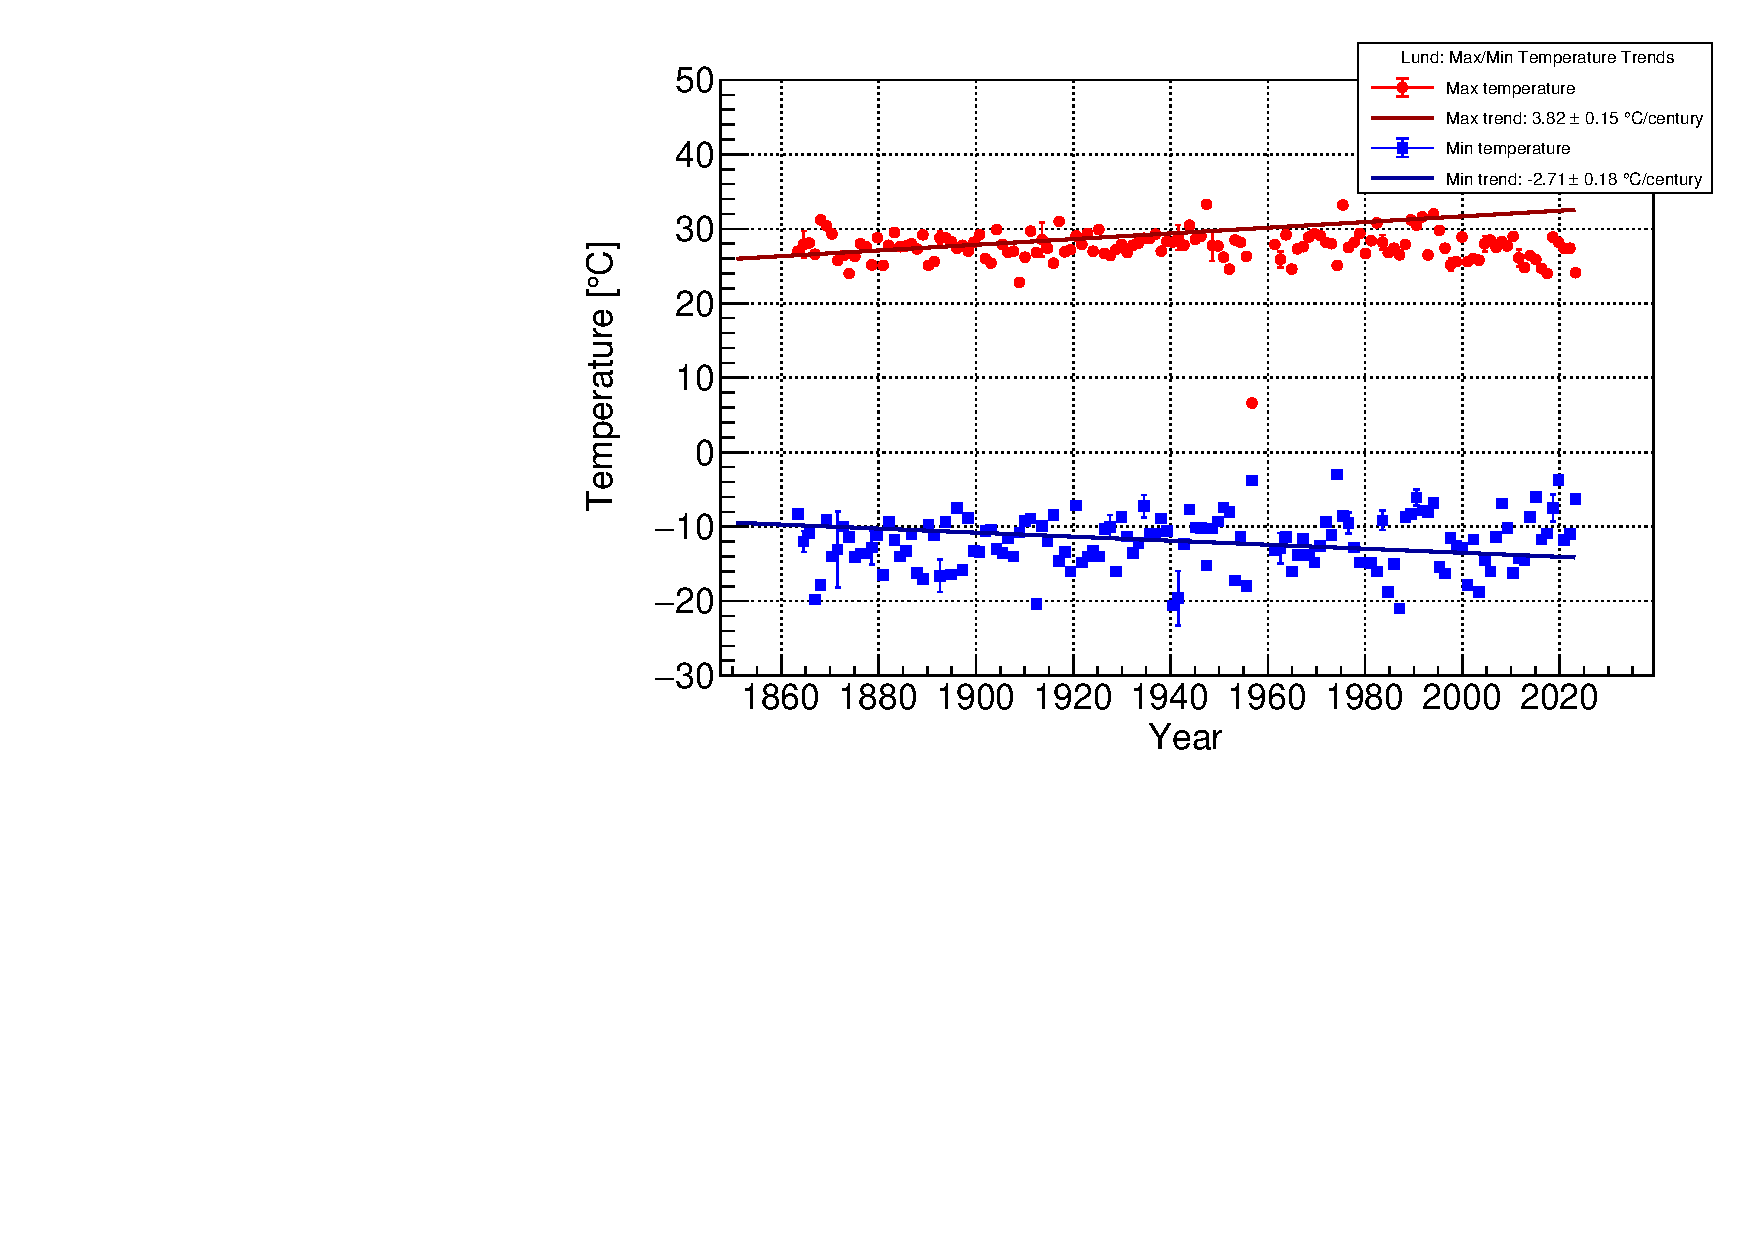
\includegraphics[width=0.9\textwidth]{plots/max_min_temps/Lund_max_min_trends.pdf}
        \caption{Long-term temperature trends at the Lund station (1850--2024). 
    Linear fits are shown for maximum and minimum temperatures. The fits shows an increase in maximmum annual temperature of about four degrees per century and a decrease in minimun annual temperature of about three degrees per century.}
        \label{fig:lund_maxmin}
%    \end{subfigure}
\end{figure}
%    \hfill
\begin{figure}[H]
%    \begin{subfigure}[b]{0.48\textwidth}
        \centering
        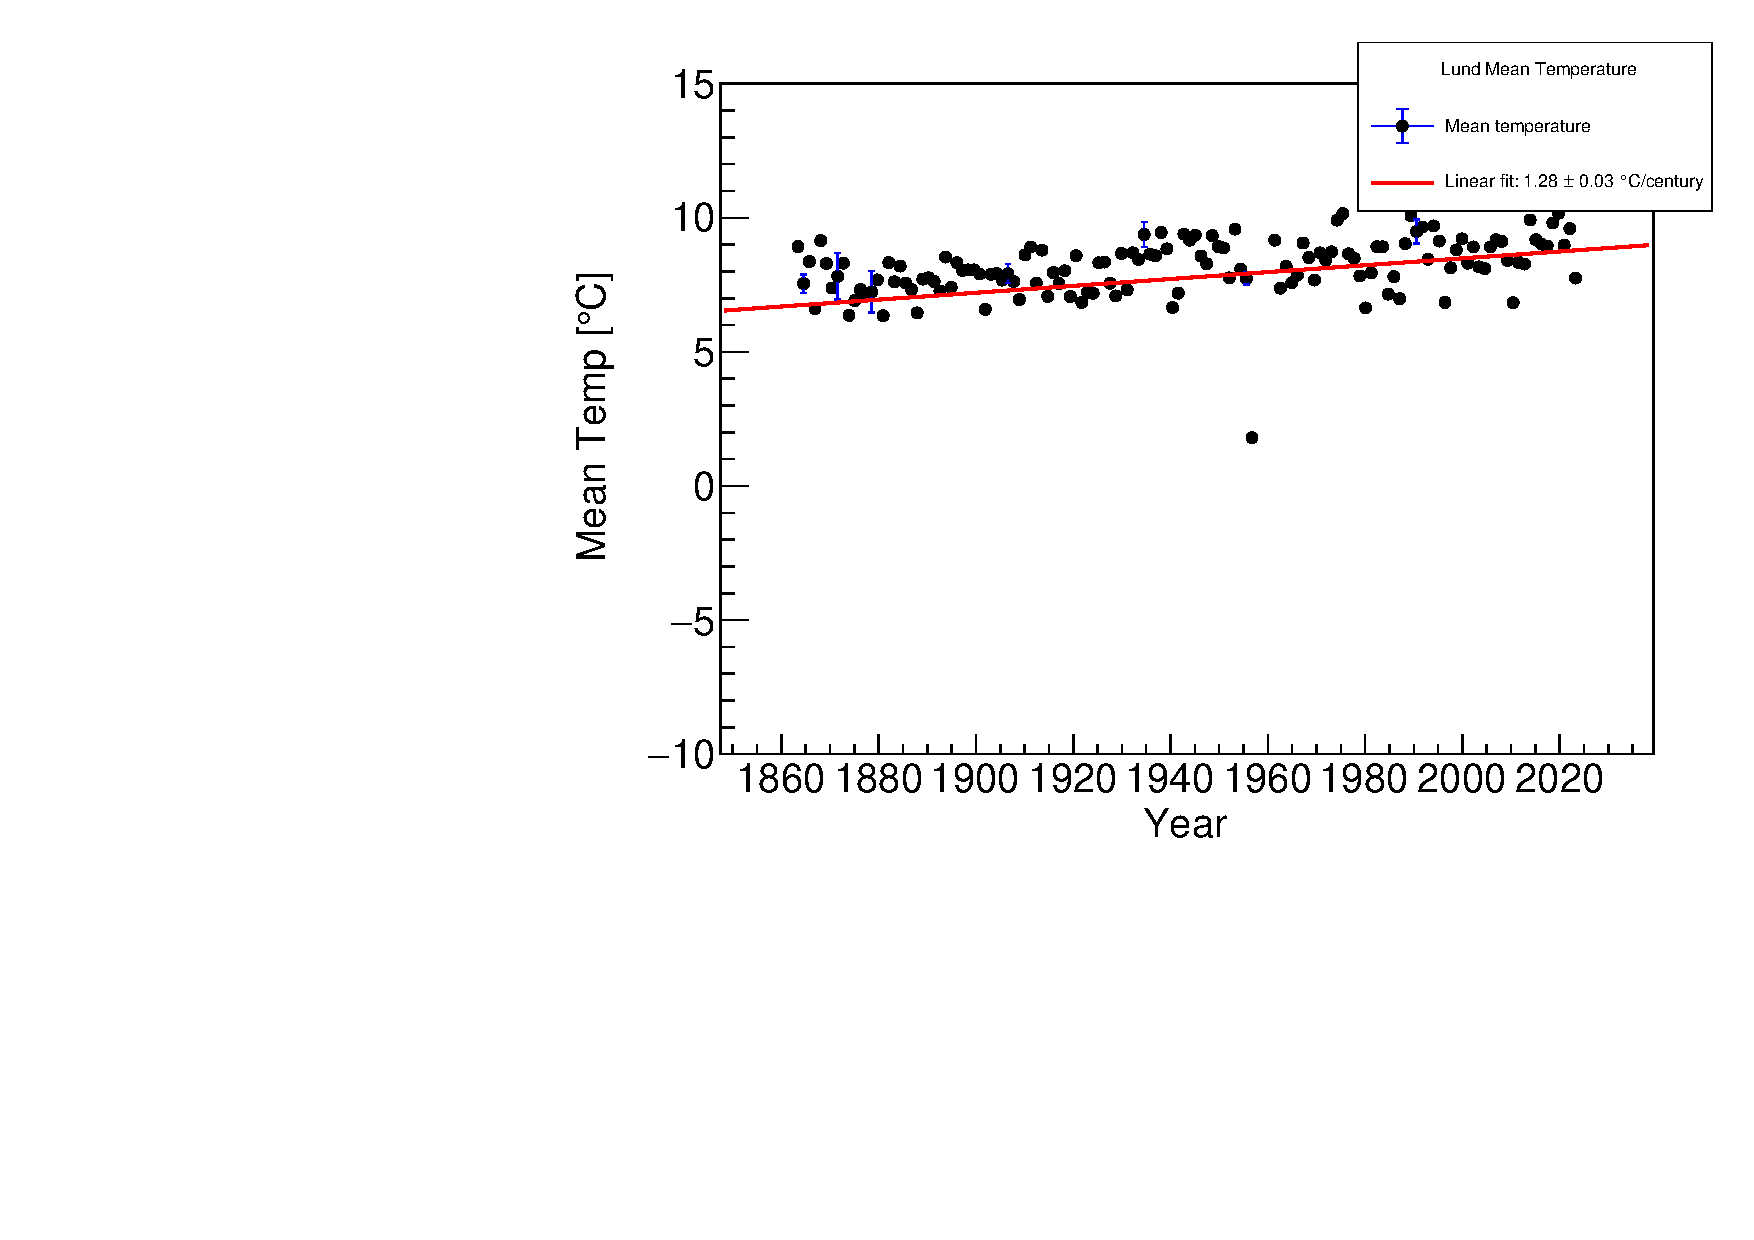
\includegraphics[width=0.9\textwidth]{plots/mean_temps/Lund_mean_trend.pdf}
        \caption{Long-term temperature trends at the Lund station (1850--2024). 
    Linear fits are shown for mean annual temperature. The fit shows an increase in temperature of about 1 degree per century.}
        \label{fig:lund_mean}
%    \end{subfigure}
%    \caption{Long-term temperature trends at the Lund station (1850--2024). 
%    Linear fits are shown for maximum, minimum, and mean temperatures.}
%    \label{fig:lund_trends}
\end{figure}


The results from multiple stations were combined to represent the general temperature trend in Sweden, as shown in Figure \ref{fig:sweden_trend}. The combined data show a positive trend, with average temperatures increasing by about one degree per century. The consistency across different stations indicates that the observed warming is not localized, but reflects a general national trend.

\begin{figure}[H]
    \centering
    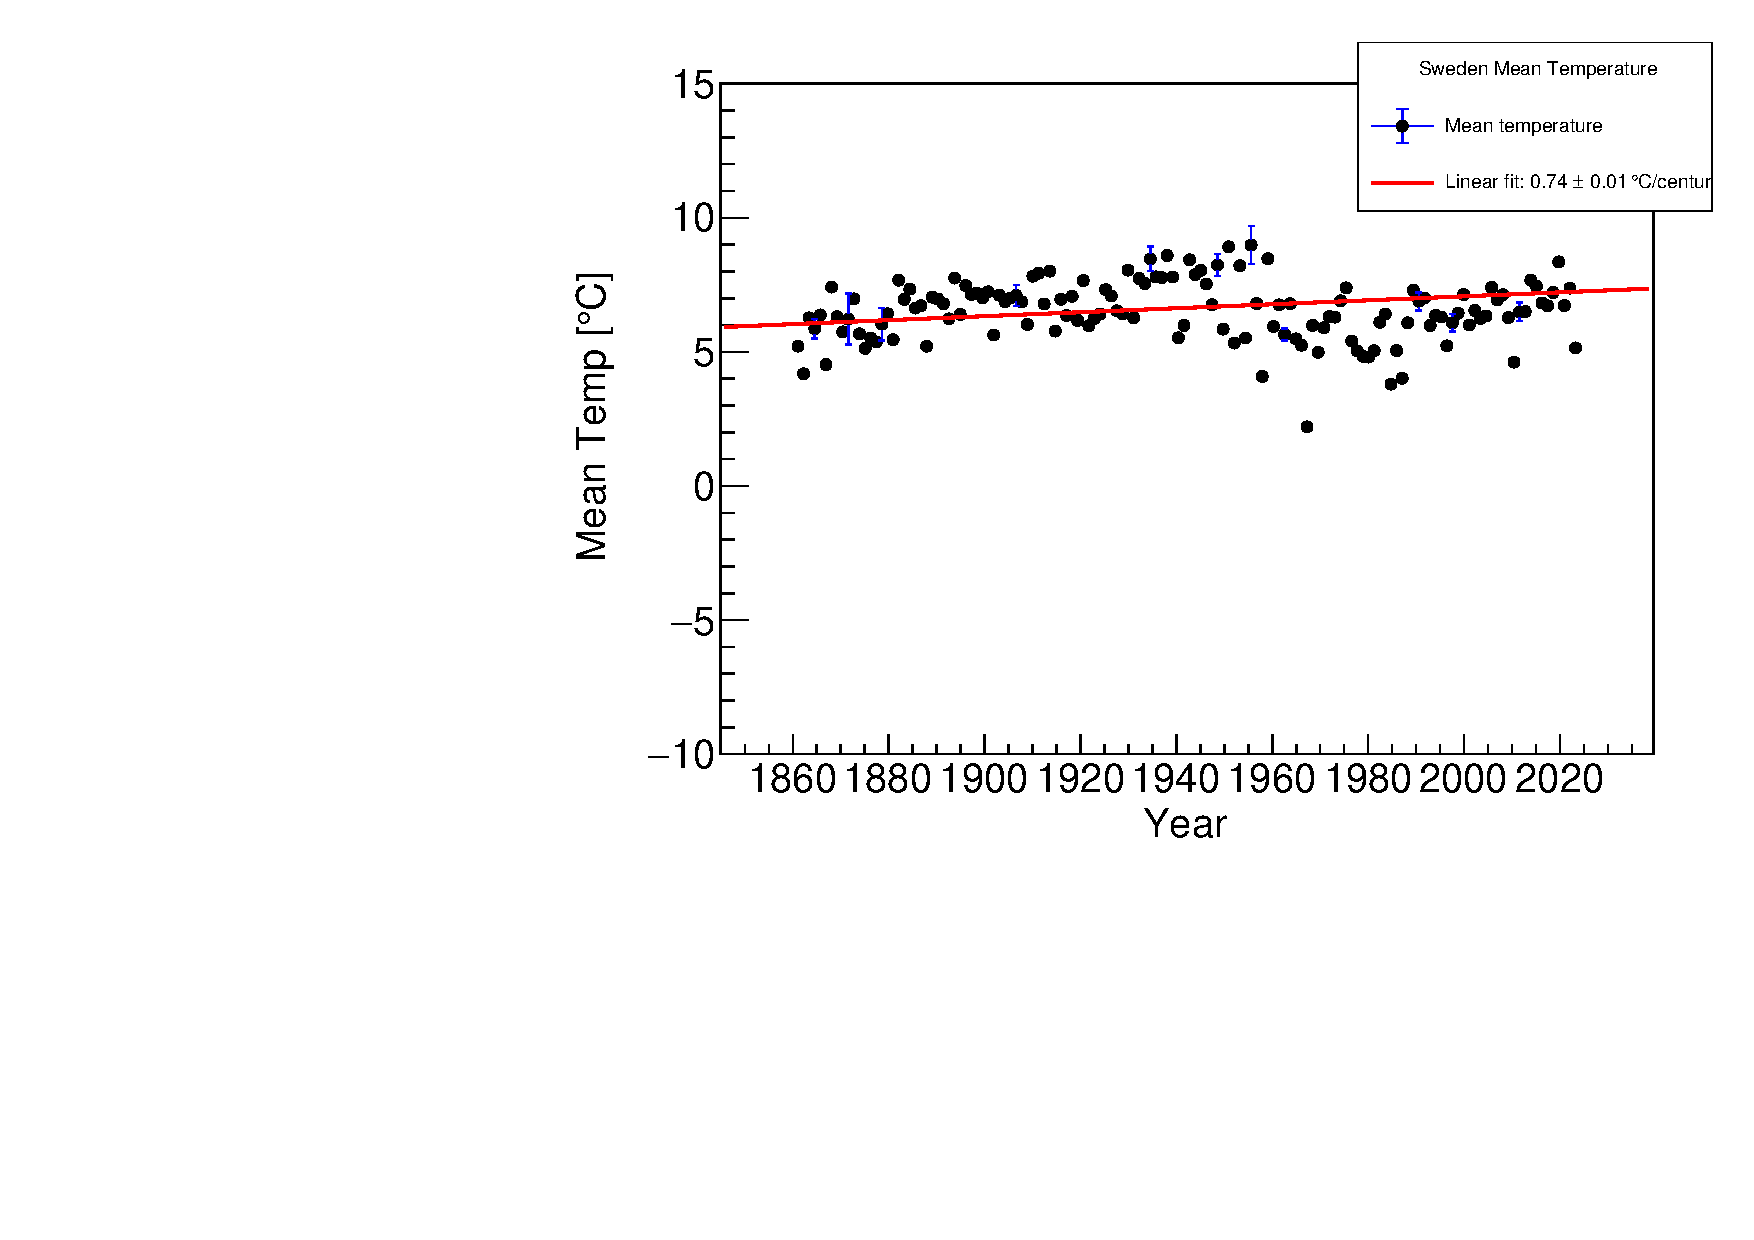
\includegraphics[width=0.9\textwidth]{plots/mean_temps/Sweden_mean_trend.pdf}
    \caption{Combined long-term temperature trend for Sweden based on multiple stations (1850--2024). The fit shows an overall warming of about one degree per century.}
    \label{fig:sweden_trend}
\end{figure}

\subsubsection{Discussion}

The temperature analysis for both the Lund station and the combined Sweden dataset shows a clear climate impact on the temperature from the mid-19th century to the present day. The linear fits for mean, maximum, and minimum temperatures all indicate slopes toward the extremes, suggesting that Sweden has experienced a gradual change in temperature over the past 170 years.

While the warming trend is consistent with global climate change observations, some local variations are visible. Lund, for example, shows slightly larger fluctuations and a stronger trend in minimum temperature, which may reflect urban heat effects or regional climate differences. The national average tends to smooth out such variations, giving a clearer picture of the overall climate trend in Sweden.

It is important to note that a linear approximation is a simplification. Temperature evolution is influenced by many factors, including natural variability, solar activity, oceanic cycles, and greenhouse gas emissions. Limited resolution and occasional data gaps, especially in older records, also introduce uncertainty in the estimated trends.

\subsubsection{Conclusion}

The analysis confirms a significant impact on the temperature trend across Sweden, with both maximum and minimum annual temperatures going toward the extremes since 1850. The results align with broader global climate observations and provide clear evidence of regional climate change effects. We can see that Sweden will experience colder winters and warmer summers, with the average temperature increasing.

For future work, more detailed modeling could include seasonal decomposition or non-linear fits to capture shorter-term oscillations and long-term variability. Combining temperature data with other meteorological parameters such as precipitation, solar radiation, or atmospheric CO$_2$ concentration would also allow for a clearer view of the driving factors behind these trends.

Overall, the study demonstrates how historical climate data and modern analysis tools like ROOT can be used to visualize and quantify long-term climate evolution in a clear and reproducible way.

\subsection{Temperature changes on our birthdays}

Figure \ref{fig:lund} and Figure \ref{fig:luleå} show the plots of the average temperatures of each day in Lund and Luleå, respectively. The plots show that the average temperature on each day follow more similar trends in Lund, compared to Luleå. It is also seen that the average temperature on 11/3 generally varies more from year to year. Looking att individual points show that if the average temperature of one day increases significantly one year, the same will happen on the other days.

\begin{figure}[H]
    \centering
    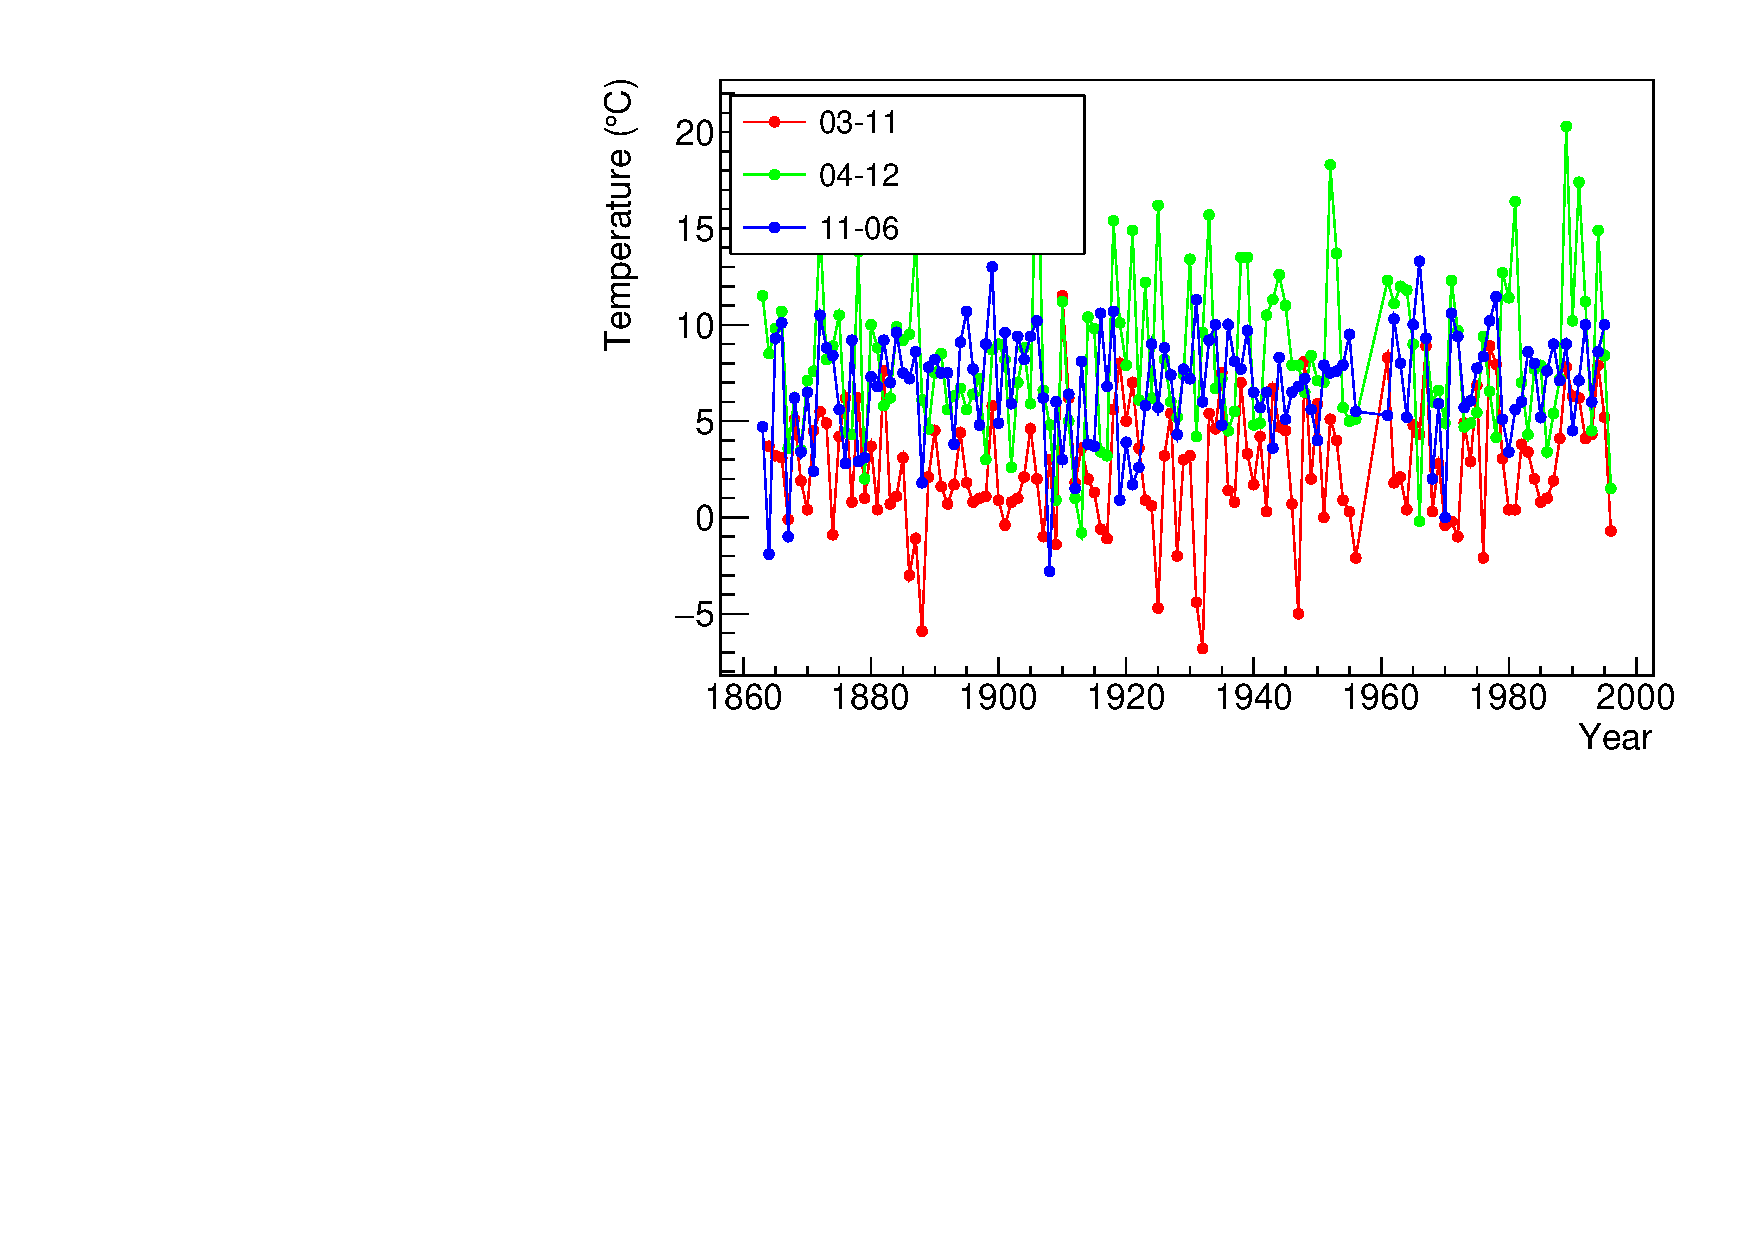
\includegraphics[width=0.85\linewidth]{../plots/bdays/Lundbdays.pdf}
    \caption{Average temperatures of the days 6/11, 12/4 and 11/3 between the years 1860 and 2000. The data was collected in Lund. The different days are labeled with different colors.}
    \label{fig:lund}
\end{figure}


\begin{figure}[H]
    \centering
    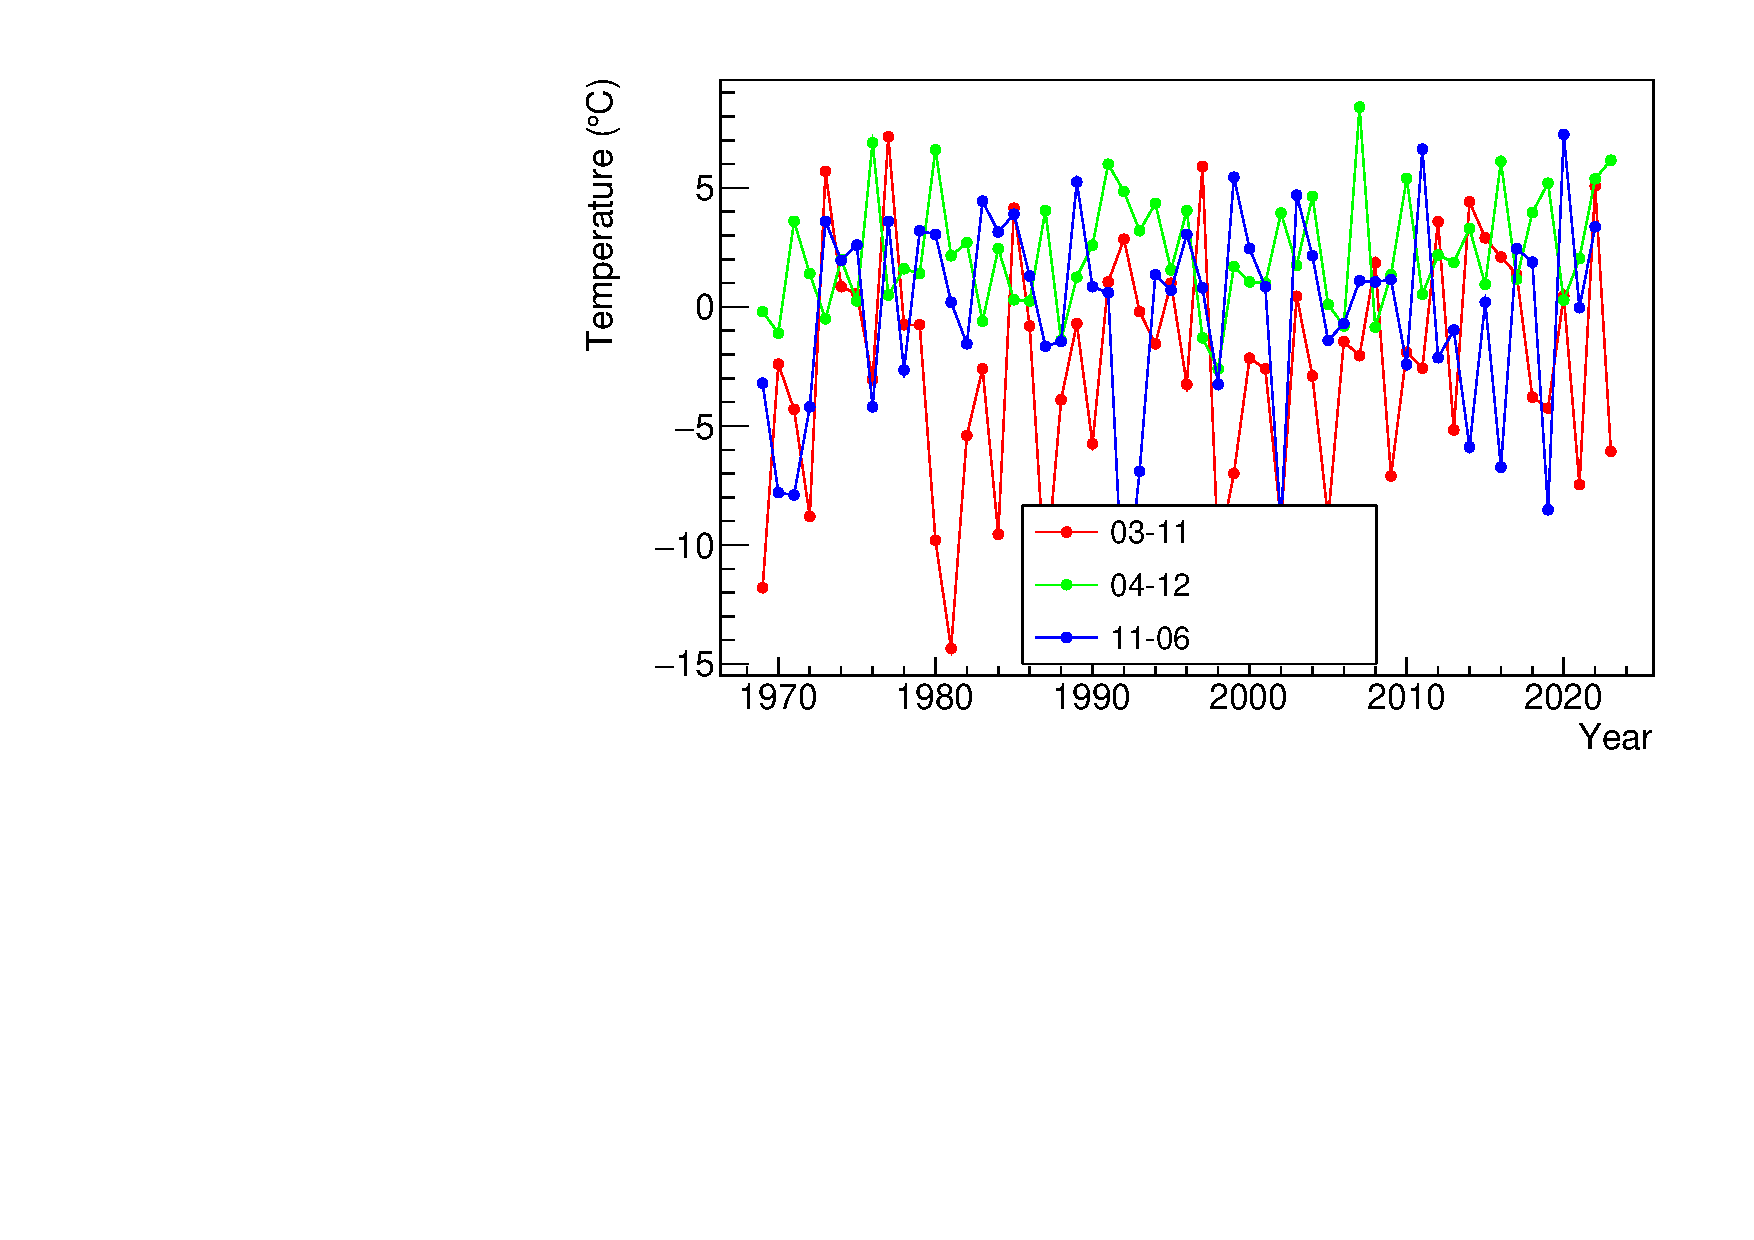
\includegraphics[width=0.85\linewidth]{../plots/bdays/Luleabdays.pdf}
    \caption{Average temperatures of the days 6/11, 12/4 and 11/3 between the years 1970 and 2025. The data was collected in Luleå. The different days are labeled with different colors.}
    \label{fig:luleå}
\end{figure}


\subsection{Discussion}
Figure \ref{fig:lund} and Figure \ref{fig:luleå} give multiple results that are worth discussing. The first result is that the average temperature each day changes in the same way each year, which is expected within the same city. However, which day that has the largest temperature change depends on the city. In Lund, the temperature seems to change the most in April and the least in November. In Luleå, it is the temperature in March that varies the most and in April it varies the least. The second clear result is that the average temperature for a specific day does not change a significant amount more than another. On temperatures all seem to increase a little bit over the years, which is expected. From another perspective, the average temperature in March and November seems to vary less during the last 15 years in Lund. The same can not be seen in Luleå but it is important to notice that the data only goes back to 1970 in Luleå. This is due to the filtering of the data before analyzing it, causing some years to not be included. This is something to consider to improve if the analysis is repeated in the future. One idea could be to have different analyses and results for different hours of the day. 

\subsection{Conclusion}
In conclusion, the analysis of the average temperature on our birthdays show no unexpected behaviour for any of the day. The variations in temperature stay consistent in each city and the recorded temperatures are expected. Both cities show a slow increase in average temperature but only Lund show less variation in temperature, especially in March and November. An important future improvement is to include the same amount of data points from each city to get a more accurate comparison. 


\subsection{Solar Activity Period Estimation}
We can see from figure \ref{fig:monthly_temp} that there is no clear trend or period in the data. It is worth pointing out that there are no values at 1 or 0 which would be expected from normalized data as the data has been averaged.

\begin{figure}[H]
    \centering
%    \begin{subfigure}[b]{0.48\textwidth}
        \centering
        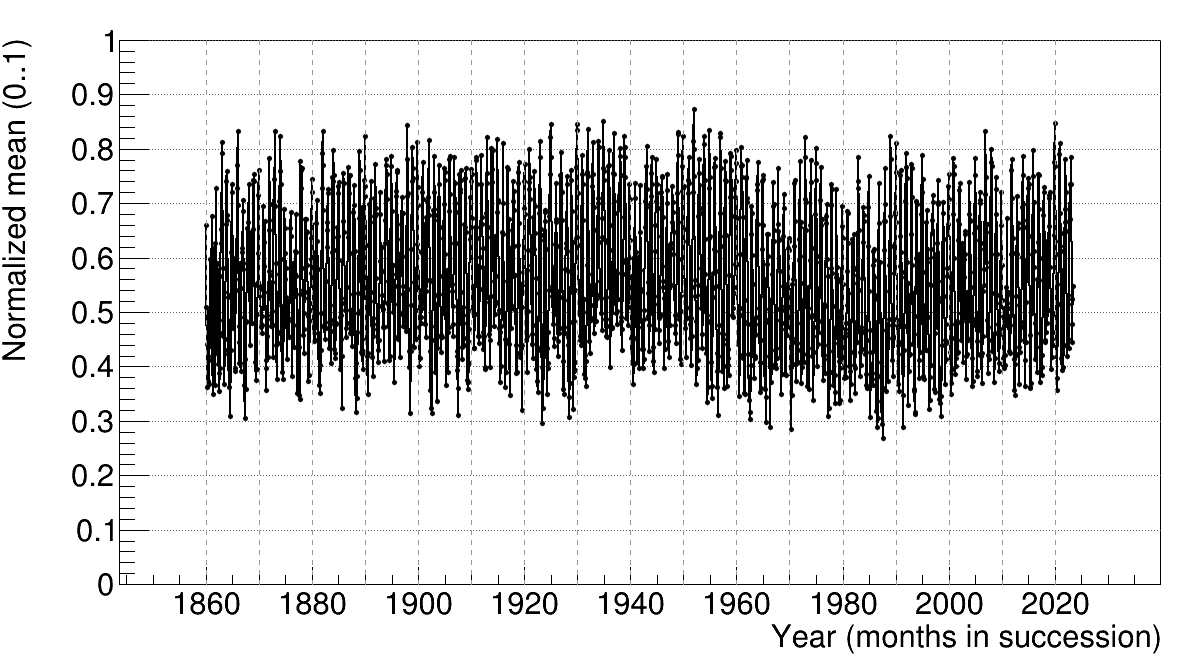
\includegraphics[width=0.9\textwidth]{plots/solar/monthly_norm_temp_timeline.png}
        \caption{This graph shows the normalized monthly temperature averaged for each month plotted in succession.}
        \label{fig:monthly_temp}
%    \end{subfigure}
\end{figure}
To be able to see what frequencies are actually relevant a fast fourier transform was done and the frequencies are plotted in \ref{fig:freq}.

\begin{figure}[H]
%    \begin{subfigure}[b]{0.48\textwidth}
        \centering
        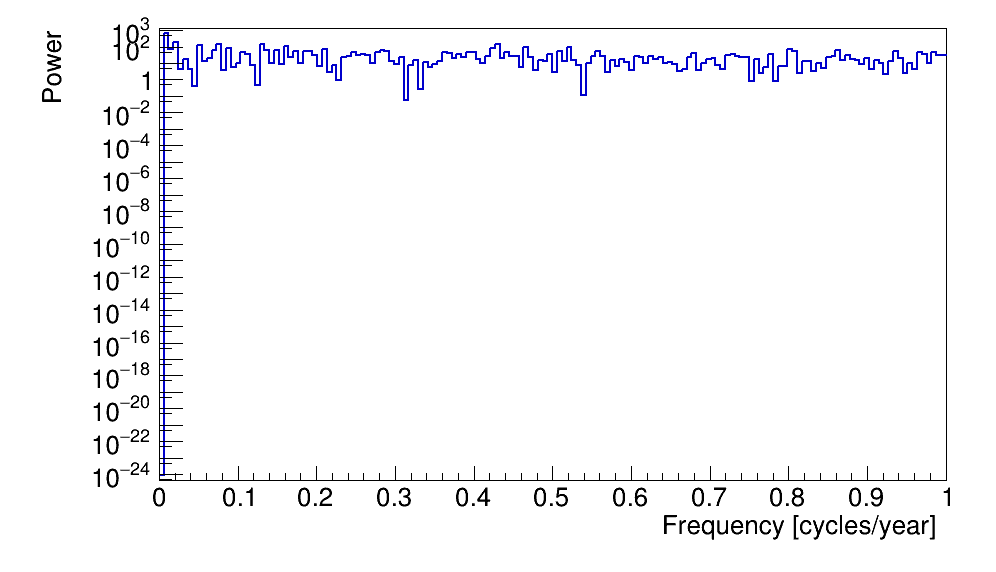
\includegraphics[width=0.9\textwidth]{plots/solar/solar_frequency_analysis.png}
        \caption{This graph shows the most relevant frequencies in the data from \ref{fig:monthly_temp}.}
        \label{fig:freq}
\end{figure}


To be able to more clearly see the actual periods, we inverted this graph to show information more clearly.

\begin{figure}[H]
    \centering
    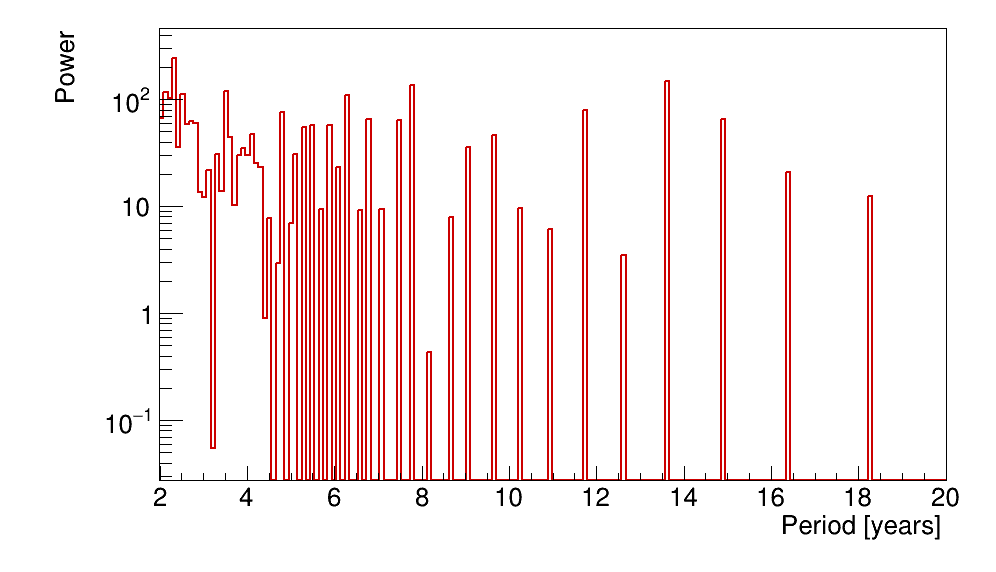
\includegraphics[width=0.9\textwidth]{plots/solar/period_analysis.png}
    \caption{periods of data in the \ref{fig:freq} graph.}
    \label{fig:period}
\end{figure}

\subsubsection{Discussion}

It is quite clear to see the data is not great. There is a lot of noise and none of the frequencies really stand out. It can quickly be looked up that the period of solar activity is around 11 years, and while \ref{fig:period} shows a peak there, the peak is pretty weak compared to everything else. This can also be seen in the \ref{fig:freq} as the frequency graph looks pretty much like a step function, with some noise. This disagrees with the original expectation that this time series would have a peak frequency in line with the known solar activity frequency.

To improve this study in the future a lot of things need to be done. Firstly data should be taken from more places around the world rather than limited to Sweden. Also meteorological effects should be taken into account as a cloudy day could mess with the data. Additionally rather than averaging every month, it may be more insightful to use a smoothing algorhithm on the data as that would remove some of the high frequency noise. Also the other sources of noise should be understood to be eliminated

\subsubsection{Conclusion}

Data disagrees with the research Question which means that either the solar cycle cannot be estimated using the temperature data, more data is needed, or data needs to be processed to a higher standard. There was a peak present at the expected 11 years, but it wasn't a major peak, indicating that it was not the most relevant in the datas frequencies.


%

\section{Discussion and Conclusion}


% Interpretation of main findings.

% How consistent are the results with expected climate trends?

% Possible sources of error (measurement gaps, station changes, etc.).

% Limitations and potential improvements (e.g., adding more stations or using homogenized data).


% Summarize main trends observed.

% Give the estimated warming rate (e.g., X °C/century).

% Mention any interesting secondary results (birthday or solar analysis).

% Reflect briefly on the learning outcomes and challenges.



%\bibliography{sample}

\end{document}
